%\documentclass[12pt]{article}
%\documentclass[a4paper, 12pt]{scrartcl}
%\voffset=-0.9in
%\hoffset=-0.6in
\documentclass[DIV=12]{article}
\setlength{\textheight}{9.1in}
\setlength{\textwidth}{7in} 
\usepackage[margin=1.1in]{geometry}
%\usepackage[justification=justified,singlelinecheck=off]{caption}



%\cofoot{\footnotesize{\rm{Pascal Grange (August 2013)}} {\rm{\ttfamily{ pascal.grange@polytechnique.org}}}}


\let\oldbibliography\thebibliography
\renewcommand{\thebibliography}[1]{%
  \oldbibliography{#1}%
  \setlength{\itemsep}{-1pt}%
{\small
\bibliography{bibfile}}
}


\usepackage[dvips]{color}
\bibliographystyle{plain}

\usepackage{graphicx}
%\usepackage{pdfpages}
%\usepackage{multicol}
%\usepackage{pstricks,pst-grad}
%\usepackage{epsfig}
\usepackage{amsmath,esint}

\newcommand{\vol}{\mathcal{V}}
\newcommand{\surf}{{\mathcal{S}}}
\newcommand{\sExt}{{{\mathcal{S}}\rightarrow{\mathrm{ext}}}}
\newcommand{\intVol}{\iiint}
\newcommand{\intSurf}{\oiint}
\newcommand{\fVol}{\overrightarrow{f^{vol}}}
\newcommand{\eBase}{(\vec{e_1}, \vec{e_2},\vec{e_3})}
\newcommand{\eBasePrime}{\left(\vec{e'_1}, \vec{e'_2},\vec{e'_3}\right)}

%\newcolumntype{S}{>{\centering\arraybackslash} m{\widthCoeff\linewidth} }

%\cofoot{\footnotesize{\rm{XJTLU, MTH308, 2014)}}}
%\title{\Huge{Research statement}\\
%    \vspace{3mm}
%       \Large{Computational biology: data analysis tools in high dimensions}}
%\author{Pascal Grange}
%\date{}
\begin{document}
%\maketitle
%\begin{flushleft}
%\Large{\bf{Research statement: data analysis tools for computational biology in high dimensions}}\\
%\large{\bf{Pascal Grange}}
%\end{flushleft}\textsc{\LARGE University of Beer}\\[1.5cm]

%\textsc{\Large Final year project}\\[0.5cm]

% Title
\title{
\noindent\hrulefill
\begin{flushleft}
{\Large \bf{XJTLU, MTH308 [Cartesian tensors and mathematical models of (elastic) solids and viscous fluids], Semester 2, 2015\\
\vspace{8mm}
\hrule
\vspace{6mm}
 Lecture 3, 17th March 2015: the stress tensor}}
\vspace{8mm}
\hrule
\vspace{6mm}
{\Large{Pascal Grange\\
Department of Mathematical Sciences\\
{\ttfamily{pascal.grange@xjtlu.edu.cn}}\\
}}
\noindent\hrulefill
\end{flushleft}}
\date{}
\author{}
\maketitle
%\noindent\hrulefill
\vspace{-3mm}

{\bf{Keywords}}. Surface forces, Cauchy stress, Stokes' theorem, balance laws.\\
\vspace{3mm}

\tableofcontents

\vspace{12mm}

\section{Volume forces and surface forces, the Cauchy  postulate}

A {\emph{volume force}} is a force that acts
 acts on a sample of matter, and is proportional to the volume of the 
 sample. Gravity is an example of volume force. On a small volume $dV$ centered\footnote{in this chapter, we take a coordinate system on $\mathbf{R}^3$ 
 with an origin $O$ and an orthonormal base $\eBase$, so we can identify the vector $\vec{x}=x_i\vec{e_i}$ to the point $M$ such that $\overrightarrow{OM}= x_i\vec{e_i}$. Moreover, we

\begin{equation}
 other equation.
 \label{otherName}
\end{equation}

 use the sum rule over repeated indices.} at point $\vec{x}$,
 a volume force is written as the product of $dV$ by the intensity  $\fVol(\vec{x})$ of the 
 force per unit volume:
\begin{equation}
 \fVol (\vec{x}) dV.
 \label{volForce}
\end{equation}
 
 I want to refer to my last Eq. \ref{volForce}.\\



 In the case of gravity, $\fVol(\vec{x}) = \rho(\vec{x}) \vec{g}$, where $\rho$ is the density 
 of the material, and $\vec{g}$ is the gravitational field.\\

 A {\emph{surface force}} is a force acting on the surface
 of a sample of matter, which is proportional to the area of the 
 surface. Cauchy postulated (in the early 19th century) that the forces
 that maintain the cohesion of a continuous medium are surface forces.
  On a small surface\footnote{By {\emph{unit normal vector}} one means a vector that is orthogonal to the surface
 and has norm 1, i.e. if $\eBase$ is an orthonormal base and $\vec{n}=n_i\vec{e_i}$, one has $n_i n_i = 1$.} centered at point $\vec{x}$, with a unit normal 
 vector $\vec{n}$, such a force is written as
\begin{equation}
 \vec{T}( \vec{x},\vec{n} ) dS,
\label{surfForce}
\end{equation}
 expressing the fact the force is proportional to the surface, depends on its 
 location (through the variable $\vec{x}$) and on its orientation (through the variable $\vec{n}$). 
Let us consider a continuous medium at equilibrium occupying the whole space (we are not 
 looking at boundaries yet), and isolate (in thought) a domain $\vol$ with boundary $\surf$ (oriented towards
 the exterior of the volume, meaning the normal vector at every 
 point of the surface points towards the exterior of the domain). If the domain $\vol$
 is at equilibrium, the volume and surface 
forces add up to zero:
\begin{equation}
\boxed{ \vec{0} = \iiint_\vol \fVol (\vec{x}) dV + \oiint_\sExt \vec{T}( \vec{x},\vec{n} ) dS.}
\label{eqEquation}
\end{equation}


\section{Stokes' theorem: reminder of the scalar version, tensor version}

 From calculus and physics you are probably familiar 
 with Stokes' theorem written in the following form:
\begin{equation}
\intVol_\vol  \frac{\partial \phi_i(\vec{x}) }{\partial x_i} dV = \intSurf_\sExt  \phi_i (\vec{x}) n_i (\vec{x}) dS
\label{stokesVec}
\end{equation}
 where $\vec{\phi}$ is a vector field (meaning there is a vector $\vec{\phi}(\vec{x})$
 at every point $\vec{x}$ in space).\\

This can be generalised to higher-order tensors. For example, if $\tau$ 
 is a tensor with two indices, the following equations  (one equation per value of $j$) hold:
\begin{equation}
  \forall j \in \{1,2,3\},\;\;\;\intVol_\vol  \frac{\partial \tau_{ji}(\vec{x})}{\partial x_i} dV = \intSurf_\sExt  \tau_{ji} (\vec{x})n_i (\vec{x})dS.
 \label{StokesTensor}
\end{equation}
 Fixing index $j$, one can just apply Stokes' theorem to the 
 vector $\vec{\phi}$ with components $\phi_1 = \tau_{j1}$, $\phi_2 = \tau_{j2}$,
$\phi_3 = \tau_{j3}$, and obtain Eq. \ref{StokesTensor}. See the 
 discussion of the Cauchy tetrahedron in the next section 
  for a geometric application. 



\section{Surface forces are a linear function of the normal vector to the surface}

In this section we are going to expose the argument due to Cauchy (about 1820),
 to prove that the vector $\vec{T}( \vec{x},\vec{n} )$
 is a linear function of the normal vector $\vec{n} = n_i\vec{e_i}$, meaning:
 \begin{equation}
\vec{T}( \vec{x},\vec{n} ) = n_i \vec{T}( \vec{x}, \vec{e_i} ).
 \label{linearityEq} 
 \end{equation}
 For definiteness let us consider that the volume forces 
 consist of gravity:
\begin{equation}
\fVol (\vec{x})= \rho(\vec{x}) \vec{g},
\label{fVolDef}
\end{equation}
 where $\rho$ is the density of the continuous medium (note that it depends on the position $\vec{x}$, since the continuous 
 medium is not necessarily homogeneous), but the result 
 would hold for any bounded volume force.\\ 

\subsection{Balance equation of a thin cylinder}
First we can establish the following lemma:
\begin{equation}
\vec{T}( \vec{x},-\vec{n} ) = -\vec{T}( \vec{x},\vec{n} ).
 \label{imparityEq}
 \end{equation}
Let us consider a cylinder of height $l$, and of radius $a$, cut by a thought experiment
 inside a continuous medium  
 as in Fig. \ref{cylinder}. Let us say that the 
 center of the upper disk is at point $M$, with $\overrightarrow{OM} = \vec{x}$,
 and that the unit normal vector to the upper disk pointing towards the exterior coincides with $\vec{n}$.
\begin{figure}
\centering
  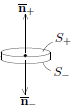
\includegraphics[width=30mm]{cylinder.png}
 \caption{A thin cylinder at equilibrium.}
\label{cylinder}
\end{figure}
 Let $\vec{n}_+$ and $\vec{n}_-$ denote the unit normal vectors
 to the upper and lower disks. These two unit vectors are opposite to each other:
 \begin{equation}
 \vec{n}_+ = -\vec{n}_-.
 \end{equation}
 If $a$ is small enough (but fixed), the dependence of $\vec{T}$ in 
 its first argument can be neglected, the density can be considered uniform (as $\vec{T}$ and $\rho$ are 
 assumed to be smooth functions), and the 
 equilibrium of the cylinder inside the continuous medium are written as:
\begin{equation}
 \vec{0}= \rho\vec{g} \pi a^2 l + \left( \vec{T}( \vec{x}, \vec{n}_+) + \vec{T}( \vec{x} - l \vec{n}_+, \vec{n}_-) \right) \pi a^2  + \intSurf_{lateral} \vec{T}( \vec{x},  \vec{n}_{lateral}) dS,
\end{equation}
 where the last term in the r.h.s  is the integral over the lateral area of the cylinder, which goes to $\vec{0}$ when $l$ goes to zero (because the integrand is bounded 
 and the lateral surface goes to zero). The first term also goes to zero when $l$ goes to zero, whereas the second term (which is the integral of 
 forces on surfaces $S_+$ and $S_-$ of Fig. \ref{cylinder}) 
  goes to  $\left( \vec{T}( \vec{x}, \vec{n}_+) + \vec{T}( \vec{x},  \vec{n}_-) \right) \pi a^2$.  As $\vec{n}_+ = -\vec{n}_-$, the limit of 
 the equilibrium condition of the cylinder when $l$ goes to zero becomes:
 \begin{equation}
\vec{T}( \vec{x},-\vec{n}_+) = -\vec{T}( \vec{x},\vec{n}_+ ),
 \end{equation}
  which is just Eq. \ref{imparityEq}. 


\subsection{Balance equation of a (small) tetrahedron}
 Let us call $M$ the point described by vector $\vec{x}$ in our reference system: $\overrightarrow{OM} = \vec{x} = x_i \vec{e_i}$.
 Let us consider a tetrahedron with one corner at $M$,
 and the three other corners $P_1, P_2, P_3$, such that 
 the vectors $\overrightarrow{MP_i}$ are parallel to the axes of the orthonormal base $\eBase$:
 \begin{equation}
 \overrightarrow{MP_1} = \epsilon y_1 \vec{e_1},\;\;\;\overrightarrow{MP_2} = \epsilon y_2 \vec{e_2},\;\;\; \overrightarrow{MP_3} = \epsilon y_3 \vec{e_3},
 \end{equation}
 and $\epsilon$ 
 For commodity the three parmeters $y_i$, for $i$ in $\{1,2,3\}$ have been chosen to be positive (this can always be ensured upon 
 choosing the axes, see Fig. \ref{tetrahedron}). 
The parameter $\epsilon$ is a positive number which we will eventually let go to zero\footnote{$\epsilon$ has no unit, it is just a number, so when $\epsilon$ goes to zero the tetrahedron 
 becomes very small, and all its points become very close to $M$, but the tetrahedron keeps the same shape.},
 to use the fact that the volume forces scale as $\epsilon^3$, while the surface forces scale as $\epsilon^2$.
 The tetrahedron is filled by the continuous medium and it is at equilibrium,
 so if we take $\vol$ to be the tetrahedron and $\mathcal{S}$ to be the surface of the tetrahedron, we have 
 the following equation:
\begin{equation}
 \intVol_{\vol} \fVol( \vec{y}) dV  +  \oiint_{\sExt} \vec{T}( \vec{y},\vec{n}(\vec{y} )) dS = \vec{0}.
\label{CauchyEq}
\end{equation}
 As $\vec{x}$ is reserved as a notation for the fixed vector $\overrightarrow{OM}=\vec{x}$ in this section,
 we use $\vec{y}$ as the integration variable (describing the  position of points inside the tetrahedron). 
 To complete the argument we need to do some geometry.\\

 The surface integral consists of four terms, one per face of the tetrahedron.
 The unit normal vectors (oriented towards the exterior of the tetrahedron) to the faces $MP_1P_2$, $MP_2P_3$ and $MP_1P_3$ are 
 the vectors $-\vec{e_3}$, $-\vec{e_1}$ and  $-\vec{e_2}$ respectively, and the areas of these faces are $ \epsilon^2(y_1y_2)/2$,
  $\epsilon^2(y_2y_3)/2$ and  $\epsilon^2(y_1y_3)/2$ respectively. Let us denote by $\vec{n} = n_i \vec{e_i}$
 the unit normal vector to the oblique face $P_1P_2P_3$ oriented towards the exterior of the tetrahedron (see Fig. \ref{tetrahedron}), and by $S_\epsilon$
 its area. By applying Pythagoras theorem one can show that $S_\epsilon = \epsilon^2 S(1)$ (where $S(1)$ is the value of the area of the
 oblique face when $\epsilon = 1$, and depends only on $y_1, y_2, y_3$).\\

\begin{figure}
  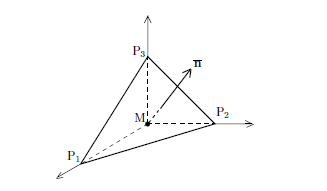
\includegraphics[width=70mm]{tetrahedron.png}
 \centering
 \caption{The Cauchy tetrahedron.}
\label{tetrahedron}
\end{figure}
 Let us denote by $C$ the center of the oblique face $P_1P_2P_3$, and by $C_3$, $C_1$, $C_2$ the centers 
 of faces $MP_1P_2$, $MP_2P_3$ and $MP_1P_3$. The volume $V_{MP_1P_2P_3}$ of the tetrahedron equals a third of  the product of the 
 surface of the base by the height (the numerical factor of $1/3$ is not so important, we will be mostly interested in the power of $\epsilon$):
\begin{equation}
V_{MP_1P_2P_3} = \frac{1}{3}\times\frac{\epsilon y_1\times \epsilon y_2}{2} \times \epsilon y_3 = \epsilon^3 \frac{y_1 y_2 y_3}{6},
\end{equation}
We are going to use the continuity of  $\fVol$  and $\vec{T}$ w.r.t. the variable $\vec{x}$ (all forces are always assumed to have derivatives, in particular they are continuous),
  as the points $C$, $C_1$, $C_2$ and $C_3$ all go to $M$ when 
 $\epsilon$ goes to zero. At leading order in $\epsilon$, the volume term in the balance equation is therefore:\\
\begin{equation}
 \intVol_{\vol} \fVol ( \vec{y})dV =  \fVol(\overrightarrow{OM}) \frac{y_1 y_2 y_3}{6}\epsilon^3 + o(\epsilon^3),
\end{equation}
while the surface term reads
\begin{equation}
 \oiint_{\sExt} \vec{T}( \vec{y},\vec{n} ) dS = \left( \vec{T}(\overrightarrow{OM}, \vec{n} ) S(1) +  \vec{T}(\overrightarrow{OM}, -\vec{e_1} )\frac{ y_2y_3 }{2}+
              \vec{T}(\overrightarrow{OM}, -\vec{e_2} )\frac{ y_1y_3 }{2}+  \vec{T}(\overrightarrow{OM}, -\vec{e_3} ) \frac{y_1y_2 }{2}\right)\epsilon^2 + o(\epsilon^2).
\end{equation}
 Because the normal vector $\vec{n}$ does not depend on $\epsilon$. So the leading order in $\epsilon$ of the balance equation 
 is just a linear combination of values of the function $\vec{T}$ at the same point in space, but different 
 value of the normal vector:
\begin{equation}
  \vec{T}(\overrightarrow{OM}, \vec{n} ) S(1) +  \vec{T}(\overrightarrow{OM}, -\vec{e_1} ) \frac{y_2y_3}{2} +
              \vec{T}(\overrightarrow{OM}, -\vec{e_2} )\frac{ y_1y_3}{2} +  \vec{T}(\overrightarrow{OM}, -\vec{e_3} )\frac{ y_1y_2}{2} = \vec{0}.
\label{CauchyEq1}
 \end{equation}
 

 Let us express the vector $\vec{n}$ in terms of our geometric data. 
 We can apply Stokes' theorem (Eq. \ref{StokesTensor}) to the Kronecker symbol:
  $\tau_{ij} (\vec{x})= \delta_{ij}$ (the value is uniform, independent from 
 $\vec{x}$), and to the tetrahedron. The integral over the volume is zero because the tensor has no dependence
 over the point, and the surface integral is just the integral of the normal vector
 over the surface, which can readily be expressed in terms of our notations:
 \begin{equation}
 \vec{0} = S(1) \vec{n} -  \frac{1}{2}\left(  y_2y_3 \vec{e_1}
    +   y_1y_3\vec{e_2}
     +  y_1y_2\vec{e_3}
   \right).
 \end{equation}
 Taking dot-products of this equation with vectors $\vec{e_1}$,  $\vec{e_2}$,  $\vec{e_3}$,
 one obtains the following relations between the components of the vector $\vec{n}$ and the
 geometric parameters of the problem:
 \begin{equation}
 S(1) n_1 =\frac{1}{2}  y_2y_3,\;\;\;  S(1) n_2 =  \frac{1}{2}y_1y_3,\;\;\; S(1) n_3 =\frac{1}{2} y_1y_2.
\label{sneqs}
\end{equation}
 Hence we can rewrite Eq. \ref{CauchyEq1}, letting components of $\vec{n}$ appear:
\begin{equation}
 \vec{0} = \vec{T}(\overrightarrow{OM}, \vec{n} ) S(1)+  \left( \vec{T}(\overrightarrow{OM}, -\vec{e_1} ) S(1)n_1
+ \vec{T}(\overrightarrow{OM}, -\vec{e_2} )S(1) n_2
  + \vec{T}(\overrightarrow{OM}, -\vec{e_3} ) S(1) n_3
   \right) 
\label{CauchyEq}
 \end{equation}
Dividing by $S(1)$ and applying Eq. \ref{imparityEq} we obtain:
\begin{equation}
\vec{0}=  \vec{T}(\overrightarrow{OM}, \vec{n} ) - \vec{T}(\overrightarrow{OM}, \vec{e_1} ) n_1
 - \vec{T}(\overrightarrow{OM}, \vec{e_2} ) n_2
  - \vec{T}(\overrightarrow{OM}, \vec{e_3} ) n_3.
\label{CauchyEq}
 \end{equation}
 Remembering that $\vec{x}= \overrightarrow{OM}$, we can rewrite this as: 
 \begin{equation}
 \vec{T}(\vec{x}, \vec{n} ) = n_j \vec{T}(\vec{x}, \vec{e_j} ),
 \end{equation}
 which is the linearity in the vector $\vec{n}$ we wanted to establish. The matrix 
  of the linear application is called the stress tensor (it depends on the point $\vec{x}$, so it can be called a 
 tensor {\emph{field}}). It is denoted by $\sigma(\vec{x})$:
 \begin{equation}
\boxed{
  \vec{T}(\vec{x}, n_j\vec{e_j} ) = \sigma_{ij}( \vec{x}) n_j \vec{e_i}.}
\label{sigmaDef}
 \end{equation}

\section{Balance equations for a continuous medium}

\subsection{Forces sum to zero}
 Even though we have started from an equilibrium equation consisting 
 of a volume integral and a surface integral, we can rewrite it as 
 a volume integral thanks to the linearity of force surfaces in the normal (the existence of the stress tensor),
 and Stoke's theorem. Indeed, Eq. \ref{sigmaDef} allows us to rewrite the equilibrium condition of Eq. \ref{eqEquation}
 as 
 \begin{equation}
 \intVol_{\vol}   f^{vol}_i( \vec{x})  dV +  \iint_\sExt \sigma_{ij}( \vec{x} ) n_j( \vec{x}) dS =  0,
\end{equation}
 where $f^{vol}_i = \fVol . \vec{e_i}$ is the component of the volume force density 
 along vector $\vec{e_i}$, and Stoke's theorem yields 
%Consider a continuous medium at equilibrium, occupying a domain $\vol$, on which volume forces
% with density  $\fVol$ are acting. The sum of these forces and the surface forces must equal zero 
 %for the medium to be at equilibrium:
\begin{equation}
 \intVol_{\vol} \left( f^{vol}_i ( \vec{x})  + \frac{\partial \sigma_{ij}}{\partial{ x_j}}( \vec{x})\right) dV \vec{e_i}=  \vec{0}.
\end{equation}
As the above equation holds for any volume $V$, the integrand is zero,
 and the following equilibrium equations hold:
 \begin{equation}
  \boxed{f^{vol}_i +\frac{\partial \sigma_{ij}}{\partial{ x_j}} = 0, \;\;\;\forall i\in \{1,2,3\}}
\label{volEquation}
 \end{equation}

\subsection{Momenta of forces sum to zero, hence the stress tensor is symmetric}
 Let us express write that the momenta of volume forces and surface forces at the origin $O$ sum to zero:
\begin{equation}
 \intVol_\vol  \overrightarrow{OM} \wedge \fVol ( \vec{x})dV  + \intSurf_\sExt \overrightarrow{OM} \wedge \vec{T}(\overrightarrow{OM},\vec{n}) dS = \vec{0}.
\label{momEq}
\end{equation}
Let us denote by $\epsilon$ the order-three tensor that is totally antisymmetric 
 in all its indices\footnote{meaning for all values of indices $i,j,k$, any permutation of two indices flips the sign of the entry: 
 $\epsilon_{ijk} = -\epsilon_{jik}$,  $\epsilon_{ijk} = -\epsilon_{ikj}$, $\epsilon_{ijk} = -\epsilon_{jik}$, which implies that all 
 entries of $\epsilon$ equal 0 (when at least two indices are equal), 1 (if the indices are obtained from $(1,2,3)$ by an even number of permutations), 
or $-1$ (if the indices are obtained from $(1,2,3)$ by an odd number of permutations).} and has $\epsilon_{123}=1$ ({\bf{NB}}: in the present context, the 
 quantity $\epsilon$, which is an order-three tensor, is not to be confused with the scaling parameter used in the 
 context of the Cauchy tetrahedron, which is a single number, and was denoted by the same symbol). One can easily check
 as an exercise that the components of 
 the vector product in three dimensions are expressed by taking the tensor product of vectors with the totally antisymmetric tensor:
\begin{equation}
 ( x_j \vec{e_j} )\wedge ( y_k \vec{e_k} ) = (\epsilon_{ijk} x_j y_k) \vec{e_i}.
\label{vecProduct}
\end{equation}
 This enables us to rewrite the integrands of Eq. \ref{momEq} in terms 
 of the components $x_i$ of the vector $\overrightarrow{OM} = x_i\vec{e_i}$. The $i$-th component
 of Eq. \ref{momEq} takes the following form:
\begin{equation}
 \intVol_\vol \epsilon_{ijk} x_j f^{vol}_k ( \vec{x})dV  + \intSurf_\sExt   \epsilon_{ijk} x_j  \sigma_{kl}(\vec{x}) n_l dS = 0.
\label{momEq2}
\end{equation}
 Stokes' theorem can be applied to the surface integral:
\begin{equation}
 \intVol_\vol  \left( \epsilon_{ijk} x_j f^{vol}_k( \vec{x}) +\frac{\partial}{\partial x_l}\left( \epsilon_{ijk} x_j  \sigma_{kl}(\vec{x}) \right) \right) dV  = 0.
\label{momEq2}
\end{equation}
 The derivative w.r.t. $x_l$ gives rise to two terms:
\begin{equation}
 \intVol_\vol  \left( \epsilon_{ijk} x_j f^{vol}_k ( \vec{x})+  \epsilon_{ijk} \delta_{jl}  \sigma_{kl}(\vec{x})+  \epsilon_{ijk} x_j  \frac{\partial \sigma_{kl}(\vec{x})}{\partial x_l}\right) dV  = 0,
\label{momEq2}
\end{equation}
and the equilibrium of forces (Eq. \ref{volEquation}) can be used to reduce the integrand to just one term:
\begin{equation}
0 = \intVol_\vol  \left( \epsilon_{ijk} x_j \left(  f^{vol}_k( \vec{x}) + \frac{\partial \sigma_{kl}(\vec{x})}{\partial x_l}  \right) +  \epsilon_{ijk}  \sigma_{kj}(\vec{x}) \right) dV
 = \intVol_\vol  \epsilon_{ijk} \delta_{jl}  \sigma_{kl}  dV.
\label{momEq3}
\end{equation}
 Since this is true for any domain $\vol$, the integrand must be zero at every point $\vec{x}$, hence:
\begin{equation}
\epsilon_{ijk}  \sigma_{kj}(\vec{x}) = 0
\label{momEq3}
\end{equation}
This equation implies that $\sigma$ is symmetric. By the definition of the antisymmetric three-tensor
 $\epsilon$, if one considers $i=1$ for instance, Eq. \ref{momEq3} only has terms corresponding 
 to $j,k \in \{2,3\}$, and becomes $\sigma_{23} - \sigma_{32} = 0$. For the same reason, 
 considering $i=2$ gives rise to $-\sigma_{13} + \sigma_{13} = 0$, and considering $i=3$
  gives rise to $\sigma_{23} - \sigma_{32} = 0$. So we have established 
 the following property as a a consequence of the equilibrium of momenta
\begin{equation}
\boxed{ \sigma_{ji} = \sigma_{ij}, \;\;\; \forall i,j \in [1..3].}
\end{equation}

\end{document}
Dear Professor Wu,

 Thank you for your email. Part of my research could fit into team 1 (Data analytic and mining),
even though it is limited to data sets from neuroscience (and not meant to develop general tools
for mining of any data set). A description follows, I hope it will be useful for our case.

 Best regards,

  Pascal Grange

Research projects:
a) Neuroanatomy from "omics" data sets

 The Allen Brain Atlas (ABA) has made the expression profiles of all genes
in the mouse brain available to researchers through the internet in 2008. On the other hand, the
diversity of neurons is being studied from the genetic viewpoint (transcriptomes of cell types).
 These two genomic data sets can be used together in order to estimate where in the
brain a given type of neuron can be found. The tools of dimensionality reduction
 and optimization are crucial to the analysis of these data sets.

b) Computational identification of cliques of autism-related genes

 Curating the scientific literature on the autism-spectrum disorder gives rise to long lists
 of genes implied in autism (based on a variety of evidence). Using the genome-wide
 data of the Allen Brain Atlas, one can cluster
these genes into sets with high similarity, and visualize where in the brain these genes are expressed.
 In collaboration with Idan Menashe (Ben-Gurion University, Israel), I identified two sets
 of autism-related genes are over-expressed in the cerebellum.

c) Modeling brain-circuit topology through connectomics data

Another kind of big data in neuroscience, "connectomics", represents the wiring diagram
of the brain by tracing how elongated neurons connect different regions to each other.
 Some circuits (related to respiration and sleep for example) are well-known, but
 the entire map of the circuit for the mouse brain has only been published in 2014 by the
Allen Institute (other teams are publishing data as well). Using tools from computational topology,
 I propose to model the complexity of the connectome in terms of the number of independent loops,
and to relate the results to brain functions.
 


Achievements:
a) - Publications :
[1 ] ​P Grange, M Hawrylycz, P Mitra, (2013), Computational neuroanatomy and co-expression of genes in the adult mouse brain, analysis tools for the Allen Brain Atlas, Quantitative Biology 

[2]​ Pascal Grange, J Bohland, B Okaty, K Sugino, L Ng, Bokil, H., Nelson, S., Hawrylycz, M., Mitra, P.P., (2014), A cell-type based model explaining co-expression patterns of genes in the brain, Proceedings of the National Academy of Sciences.


- Talk at IEEE CISS 2012 (Princeton) :
Pascal Grange, P Mitra, (2012), Computational neuroanatomy and gene expression: Optimal sets of marker genes for brain regions, IEEE Conference on Information Sciences and Systems 
- Talk at NIPS Neural Information Processing Systems, (Montreal, December 2014),
in the workshop on omics data for the brain.


b) Published
​I Menashe, P Grange, E Larsen, S Banerjee-Basu, P Mitra, (2013), Co-expression profiling of autism genes in the mouse brain, PLoS Computational Biology - See more at: http://academic.xjtlu.edu.cn/maths/SitePages/StaffDetail.aspx?TermStoreId=b3eabbf4-4f09-4c6a-9193-05252181a029&TermSetId=3c579f36-ed64-47d9-bb97-b2fb68c03acc&TermId=3011dcbc-4780-4a01-9a02-cee04b901ac7&UrlSuffix=pascal-grange#sthash.By7FZASG.dpuf

 Under review in Frontiers in Computational Neuroscience:
Pascal Grange, Idan Menashe, Michael Hawrylycz 
Cell-type-specific neuroanatomy of brain-wide expression of autism-related genes


Awards:
a) and b) were initially funded in the United States by the NIH and the Simons Foundation
c) RDF from XJTLU.


